\documentclass{beamer}

% Minimal white look
\usetheme{default}
\useoutertheme{infolines}
\setbeamertemplate{navigation symbols}{}

\setbeamercolor{background canvas}{bg=white}
\setbeamercolor{frametitle}{bg=white, fg=black}
\setbeamercolor{title}{fg=black}
\setbeamercolor{title in head/foot}{bg=white, fg=black}
\setbeamercolor{author in head/foot}{bg=white, fg=black}
\setbeamercolor{date in head/foot}{bg=white, fg=black}
\setbeamercolor{section in head/foot}{bg=white, fg=black}

% Add package for positioning and hyperlinks
\usepackage{tikz}
\setbeamercolor{frametitle}{bg=white, fg=RoyalBlue}
\setbeamercolor{title}{fg=RoyalBlue}
% Add QR code to every slide (except title slides)
% \addtobeamertemplate{frametitle}{}{%
%     \begin{tikzpicture}[remember picture,overlay]
%         \node[anchor=south east,xshift=-0.5cm,yshift=0.5cm] at (current page.south east) {
%             
\includegraphics[width=1.5cm]{qr_small.png}
% Add package for positioning, hyperlinks, and colors
%     \end{tikzpicture}
% }
\usepackage[dvipsnames]{xcolor}

% Make all boldface text blue
\let\oldtextbf\textbf
\renewcommand{\textbf}[1]{\textcolor{RoyalBlue}{\oldtextbf{#1}}}

% Quick highlight helpers
\newcommand{\kwGreen}[1]{\textcolor{ForestGreen}{\oldtextbf{#1}}}
\newcommand{\kwRed}[1]{\textcolor{BrickRed}{\oldtextbf{#1}}}
\newcommand{\kwOrange}[1]{\textcolor{Orange}{\oldtextbf{#1}}}

\title[Tabulating the NHS Waiting List]{Tabulating the NHS Waiting List}

\author[ Walton,  Davis, Mohammed]{\texorpdfstring{{Neil Walton\\Durham University Business School\\ \textcolor{ForestGreen}{\href{mailto:neil.walton@durham.ac.uk}{neil.walton@durham.ac.uk}}\\\vspace{1cm}Rhian Davis, Mohammed Mohammed\\The Strategy Unit}}{Neil Walton; Rhian Davis; Mohammed Mohammed}}
\date{\today}

\begin{document}

%------------------------------------------------------------
\begin{frame}
  \titlepage
\end{frame}

%------------------------------------------------------------

\begin{frame}{Access the National Table}
    \begin{center}
        
\includegraphics[width=0.35\textwidth]{qr_small.png}
        \hspace{1cm}
        
\includegraphics[width=0.35\textwidth]{qr_strategyunit_viewer.png}
        
        \vspace{0.5cm}
        \large
        \href{https://neilwalton.github.io/National_Table/}{\qquad\qquad\footnotesize neilwalton.github.io/} \hfill
        \href{https://connect.strategyunitwm.nhs.uk/content/03d90ae5-e77f-44ba-84c2-33a25348681a/viewer-rpubs-393c5f6b37ea.html}{\footnotesize Strategy Unit Viewer Link\qquad \qquad }

        \vspace{0.5cm}
        \href{https://github.com/The-Strategy-Unit/nhs-waiting-list-explorer}{github repo link}

        \href{https://github.com/neilwalton/National_Table/blob/main/HACA_Walton.pdf}{these slides link}
    \end{center}
\end{frame}
%------------------------------------------------------------
\section{background}

\begin{frame}
  \centering
    \huge
    \textcolor{RoyalBlue}{Background}
\end{frame}
%------------------------------------------------------------
\begin{frame}
  \centering
    \large
    % \textcolor{RoyalBlue}{Background}
    \vspace{1cm}
    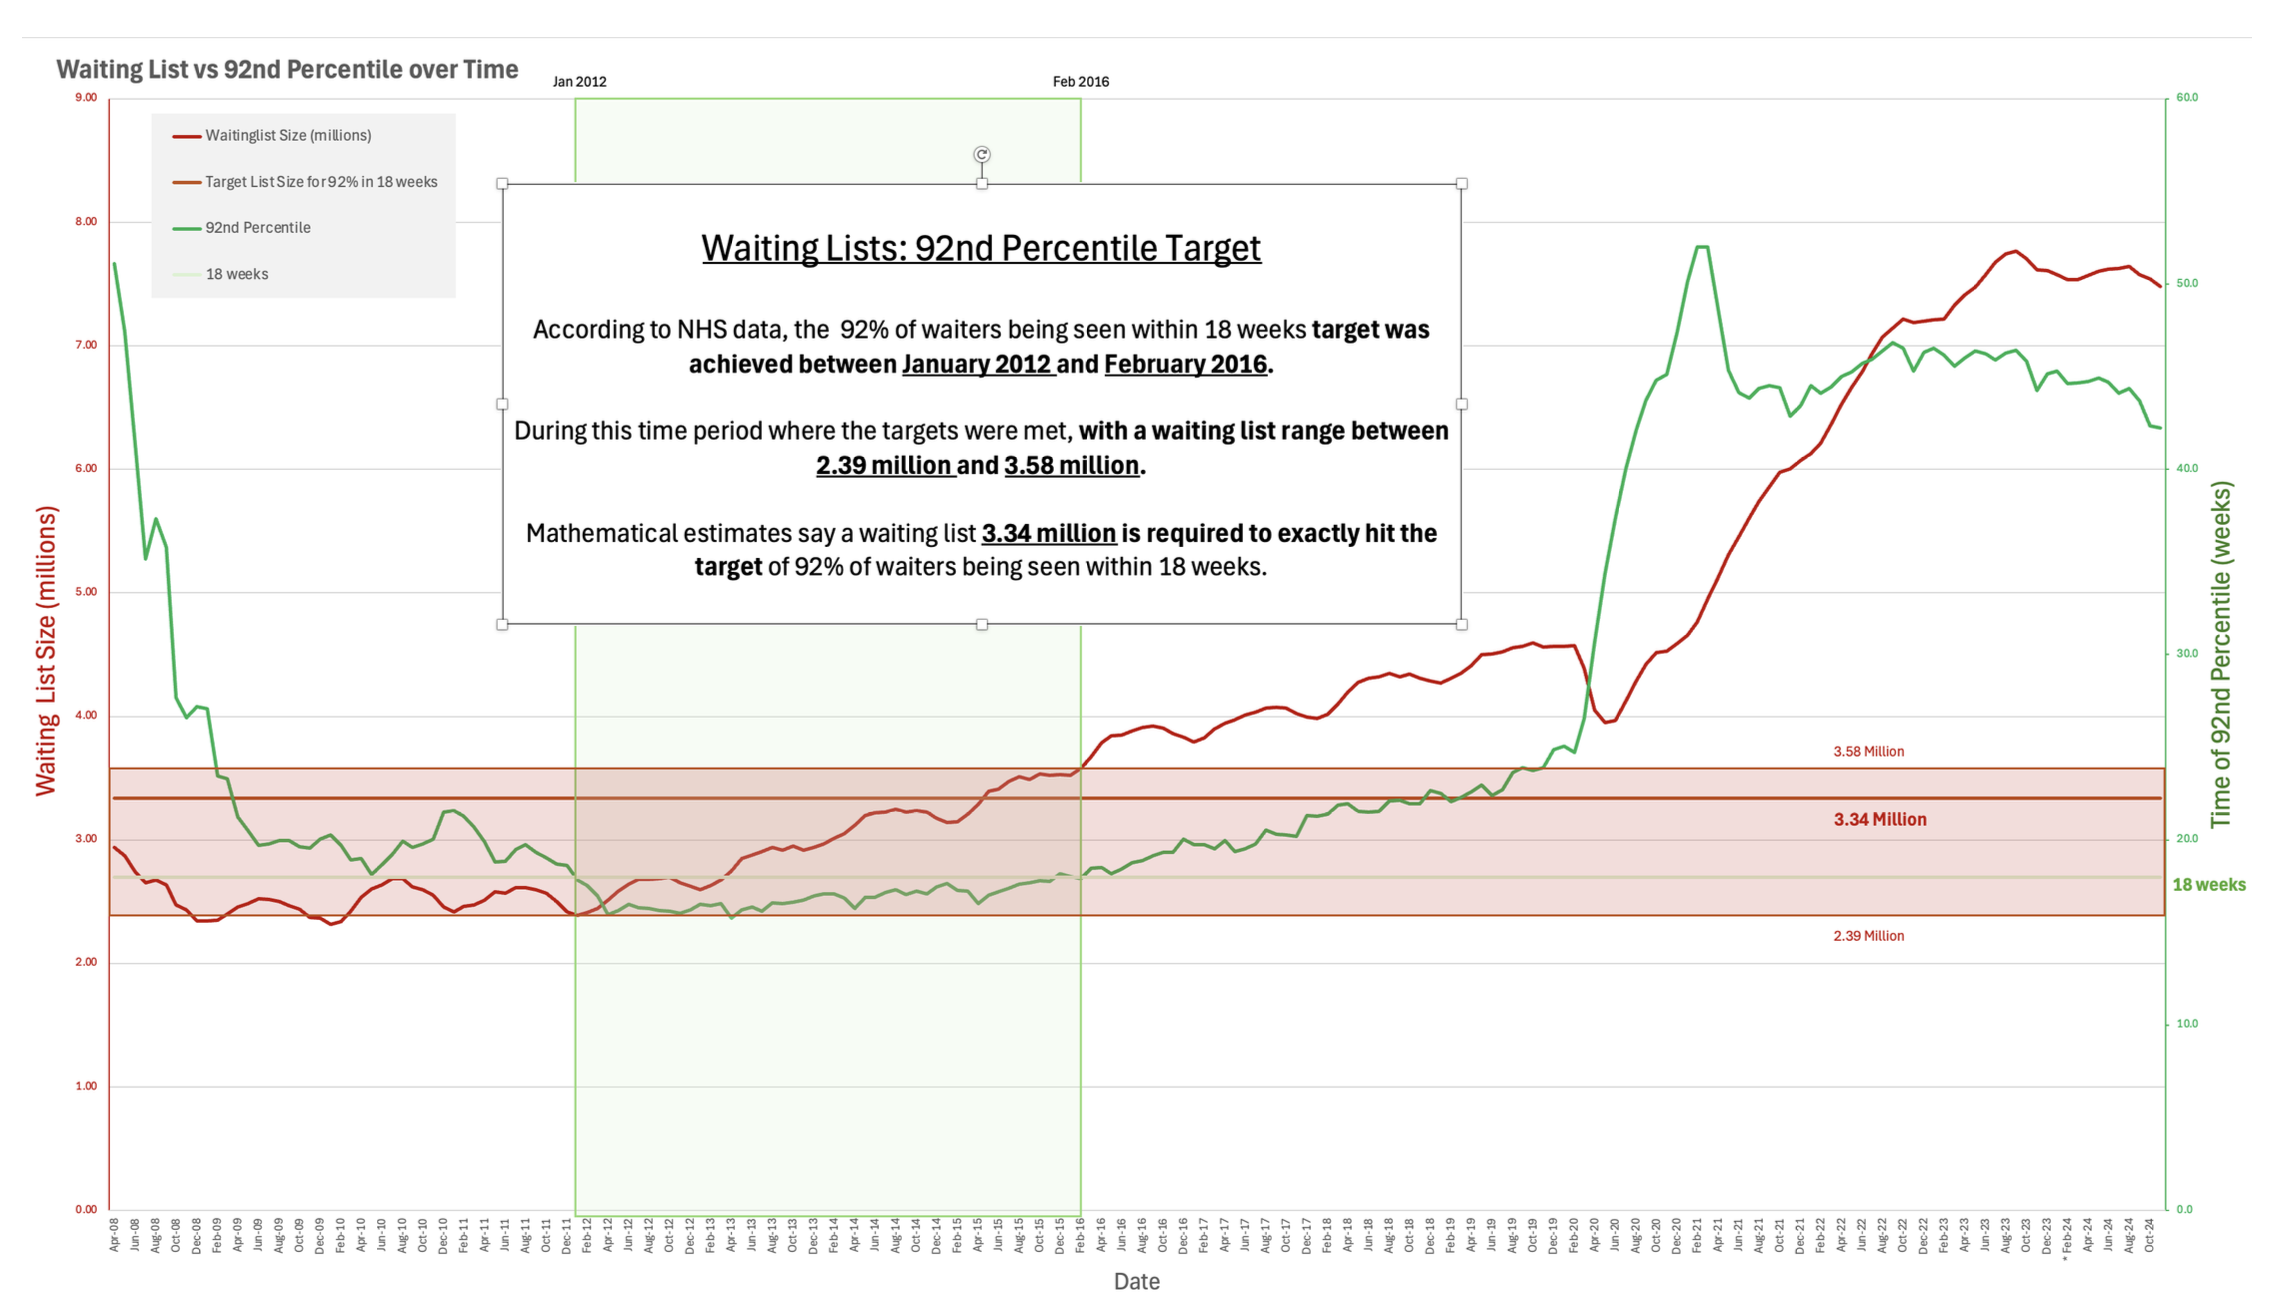
\includegraphics[width=1.\textwidth]{WL_overtime.png}
\end{frame}

%------------------------------------------------------------
\begin{frame}{Understanding Waiting Lists Pressures (2022)}

  \textbf{Paper link:}  
  \href{https://www.medrxiv.org/content/10.1101/2022.08.23.22279117v1.full}{\texttt{medrxiv.org/2022.08.23.22279117}}
\\
\textbf{YouTube explainer:}
\href{https://youtu.be/NWthhW5Fgls?si=e2LRcd9ymTyQKqrM}{\texttt{youtu.be/NWthhW5Fgls}}
\\
  \vspace{1em}
  \textbf{Why this matters}
  \begin{itemize}
    \item NHS waiting lists are under sustained pressure, with long delays for many patients.
    \item Operational managers must balance demand, capacity, and long-wait trajectories.
  \end{itemize}

  \vspace{1em}
  \textbf{What the paper does}
  \begin{itemize}
    \item Introduces a queueing-theoretic framing of waiting-list pressures:
    treatment capacity, queue size, waiting times, and the
      stability condition.
  \end{itemize}

%   \vspace{1em}
%   \textbf{Relevance to the National Table}
%   \begin{itemize}
%     \item Your long, tidy national table provides the inputs for queueing metrics:
%           arrivals, treatments, long-wait thresholds, and backlog evolution.
%     \item Enables both descriptive analysis (tabulation) and operational insight
%           (pressure, stability, capacity required).
%     \item Places national-level data into the same analytical framing used in the paper.
%   \end{itemize}

\end{frame}

\begin{frame}{NHSRwaitinglist: waiting-list analysis}

  \textbf{What is it?} 
  The R package {\tt NHSRwaitinglist}, by the NHS‑R Community, implements the queue-theoretic waiting-list methodology from Fong et al. (2022).  %[oai_citation:0‡nhs-r-community.github.io](https://nhs-r-community.github.io/NHSRwaitinglist/index.html?utm_source=chatgpt.com)  

\begin{center}
\fcolorbox{gray}{lightgray}{%
    \begin{minipage}{0.8\textwidth}
        \texttt{\textcolor{blue}{install.packages}("NHSRwaitinglist")} \\
        \texttt{\textcolor{blue}{library}(NHSRwaitinglist)}
    \end{minipage}%
}
\end{center}

  \vspace{1em}
  \textbf{Key capabilities}
  \begin{itemize}
    \item Compute all key waiting-list statistics via {\tt wl\_stats()}. % [oai_citation:1‡nhs-r-community.github.io](https://nhs-r-community.github.io/NHSRwaitinglist/reference/wl_stats.html)  
    \item Simulate waiting-list scenarios using {\tt wl\_simulator()}. % [oai_citation:2‡nhs-r-community.github.io](https://nhs-r-community.github.io/NHSRwaitinglist/articles/example_walkthrough.html)  
    \item Create capacity plan using {\tt wl\_target\_capacity()}. % [oai_citation:3‡CRAN](https://cran.r-project.org/web/packages/NHSRwaitinglist/refman/NHSRwaitinglist.html?utm_source=chatgpt.com)  
  \end{itemize}

%   \vspace{1em}
%   \textbf{Why this matters for the National Table}  
%   \begin{itemize}
%     \item Once waiting-list data are tabulated (e.g. via your “national table”), analysts can feed them into NHSRwaitinglist to derive deeper operational metrics.  
%     \item Enables scenario analysis, forecasting, backlog clearance planning — beyond static tabulations.  
%     \item Facilitates communication with managers and planners using standard metrics like load, pressure, target capacity, queue size.  
%   \end{itemize}

%   \vspace{1em}
%   \textbf{Further info / link} \\  
%   \href{https://CRAN.R-project.org/package=NHSRwaitinglist}{CRAN page for NHSRwaitinglist} — installation \& documentation. \\
%   \href{https://nhs-r-community.github.io/NHSRwaitinglist/}{NHSRwaitinglist website} — vignettes, worked examples, explanatory videos.  

\vspace{1em}
\textbf{Further info / links} \\  
\href{https://cran.r-project.org/web/packages/NHSRwaitinglist/index.html}{\texttt{CRAN link}} — installation \& documentation. \\
\href{https://nhs-r-community.github.io/NHSRwaitinglist/}{\tt  github website} — worked examples, explanatory videos.
\end{frame}

\begin{frame}{Waiting Lists Must Halve}
  \textit{From NHS England statistical press notice (Oct 10th), I believe we have around 450K RTT clockstarts a week. So this suggests the waiting list size should be
\[
7.2 * 450,000 = 3,240,00
\]
So current data suggests the waiting list should be 3,240,000 the current data suggests the waiting list is 7,600,000. I.e. the government needs to roughly half the waiting lists in the coming term to meet its target.} %Late '24

\medskip
\textcolor{RoyalBlue}{An advanced numerical model:}

``The NHS waiting list in England must halve to reach waiting time targets" Wood, Fox, Morgan, Walton, 2025.

\medskip
Morning Star; LBC; Independent; Telegraph; Spectator

\end{frame}

\begin{frame}{National Waiting List Conference}
\centering
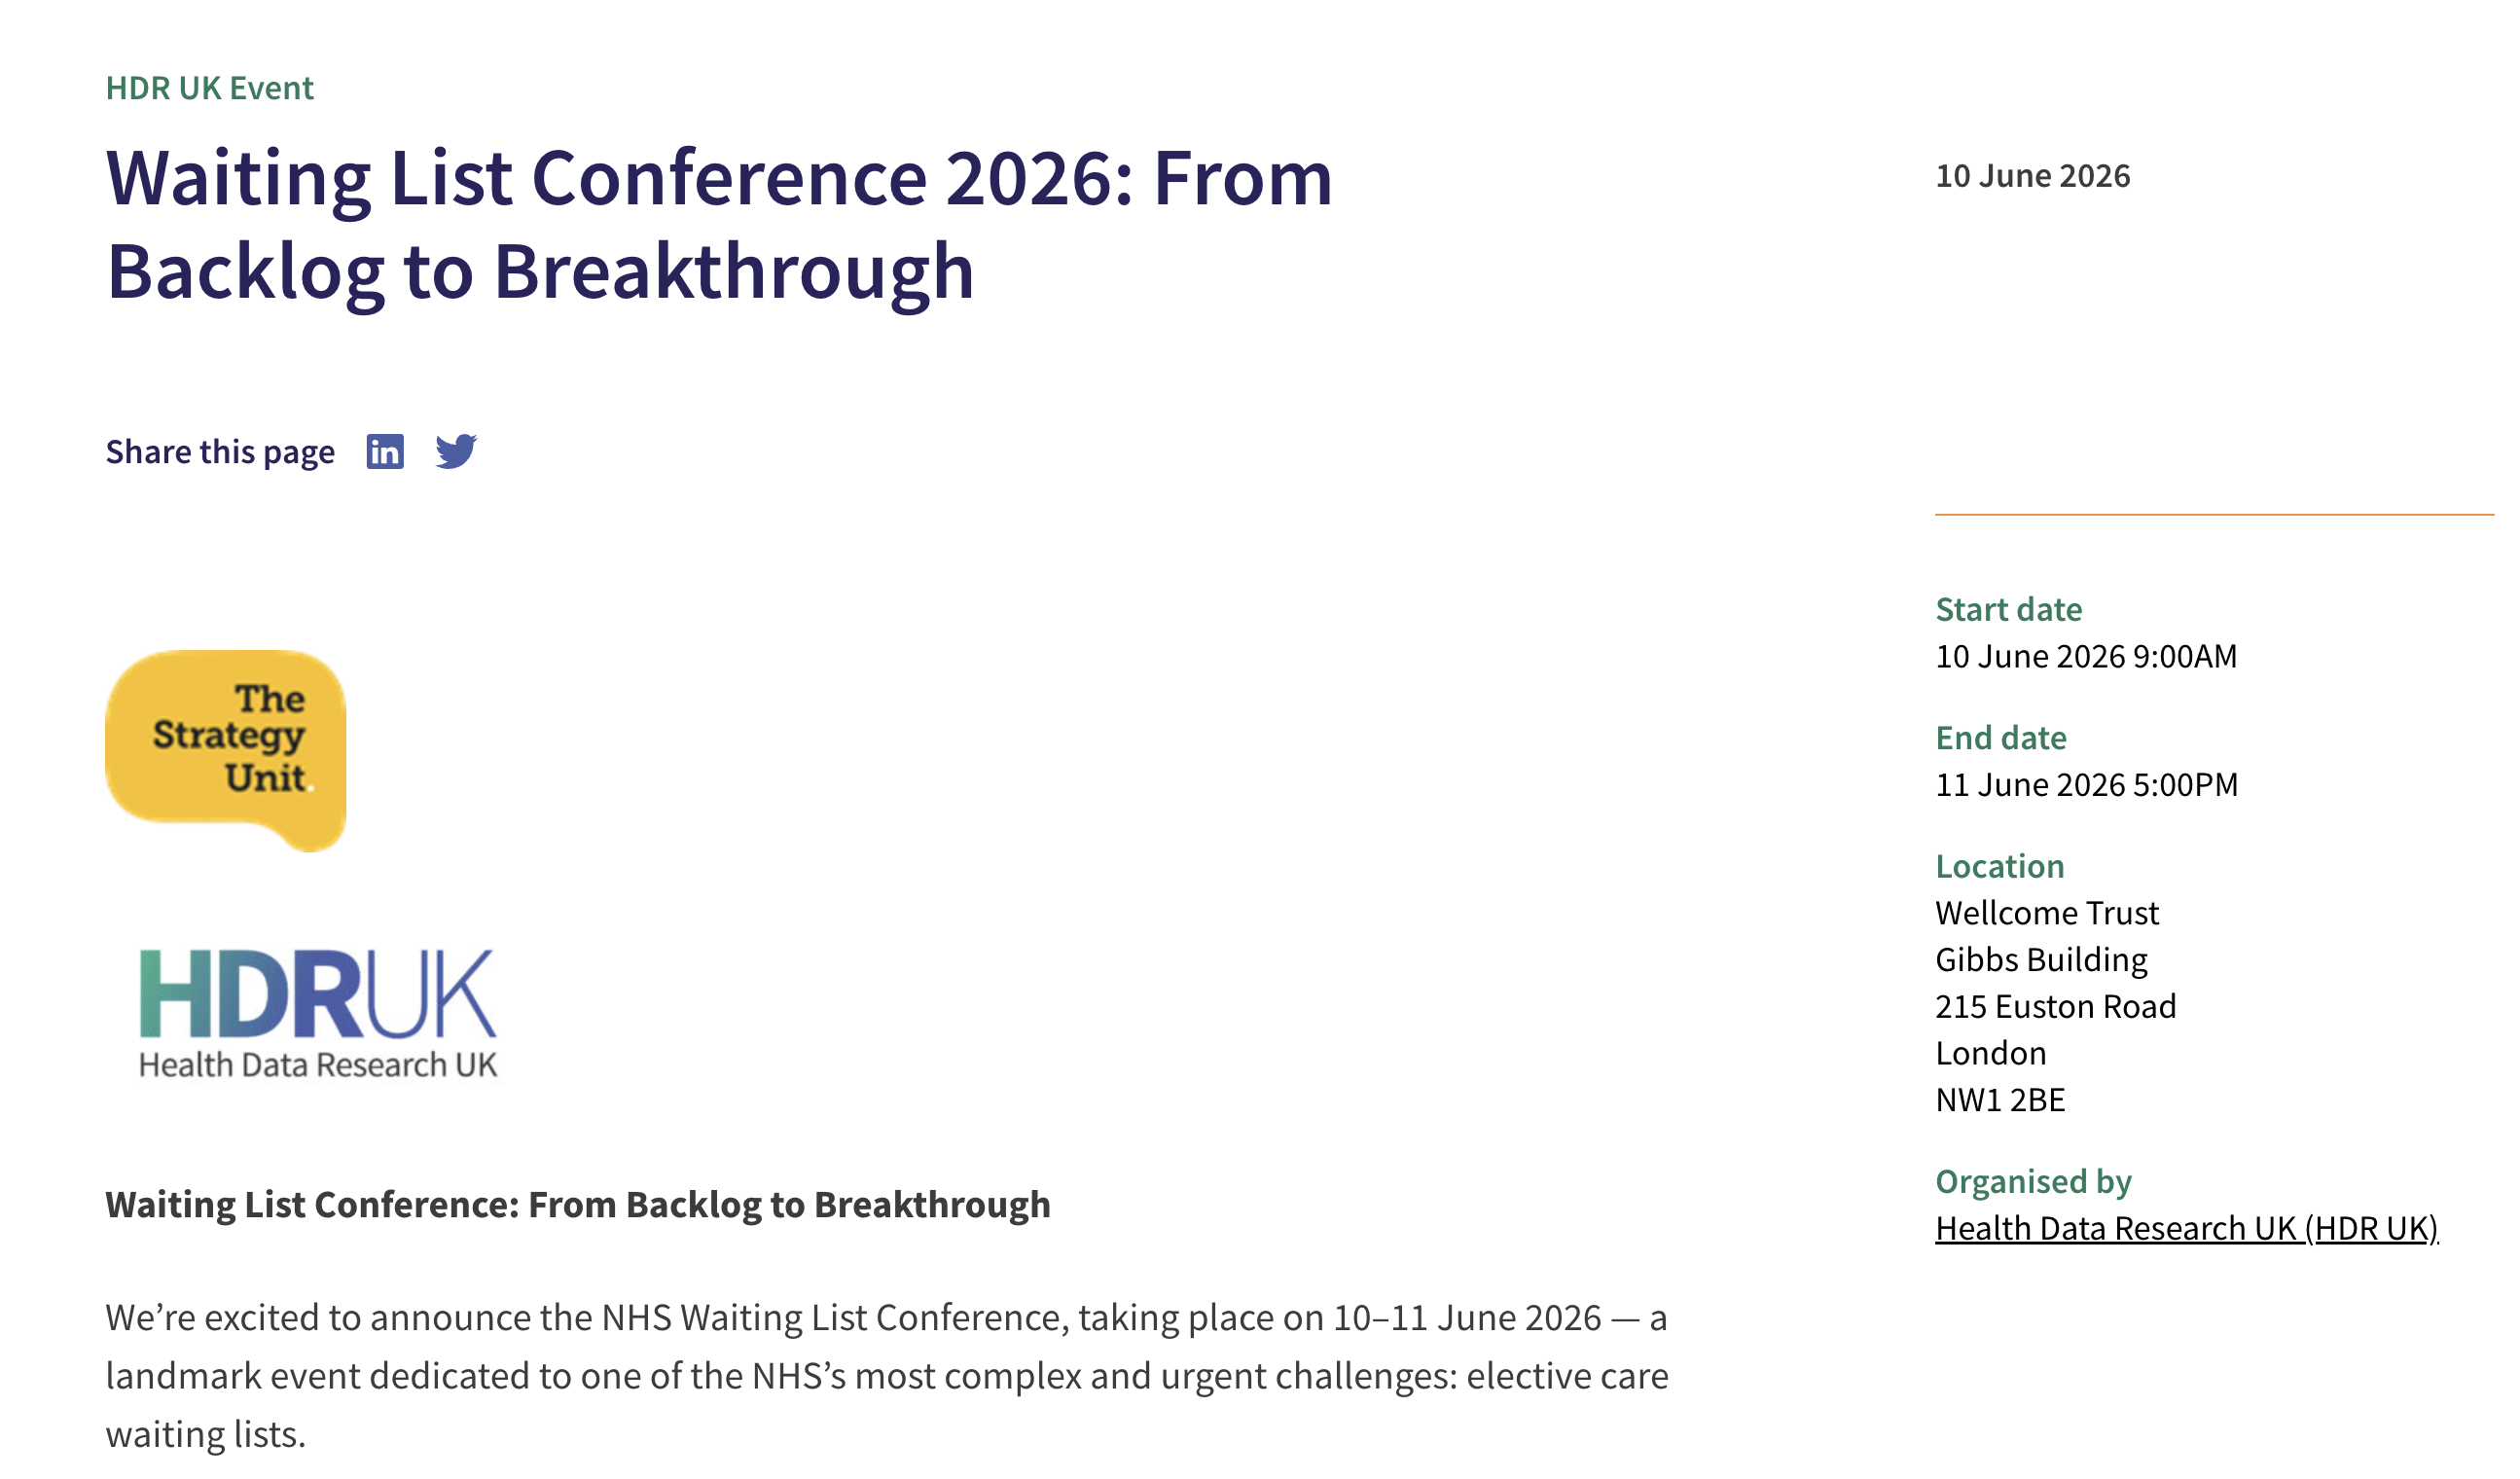
\includegraphics[width=0.9\textwidth]{Waiting_List_Conference.png}

\href{https://www.hdruk.ac.uk/events/waiting-list-conference-2026-from-backlog-to-breakthrough/}{\textbf{Conference Site Link}} \qquad / \qquad 
\href{https://forms.office.com/Pages/ResponsePage.aspx?id=saxMhCdwY0Kdihj6pb8IOdcZpXsErBVHoko2MOuOEtRUMVFPUEtGUVk4RUxLTlFGU1M1VVBIOVFCTy4u}{\textbf{Abstract Submission Link}}
\end{frame}



\section{The National Table}


\begin{frame}
  \centering
    \huge
    \textcolor{RoyalBlue}{The National Table}
\end{frame}



\begin{frame}{Motivation}
  \begin{itemize}
    \item NHS waiting lists have reached historically high levels.
    \item The underlying data are published, but not always easy to interrogate.
    \item Policy questions typically require slicing by:
      \begin{itemize}
        \item organisation (trust / system),
        \item specialty or treatment function,
        \item type and duration of wait.
      \end{itemize}
    \item Aim: build a single, transparent ``National Table'' that
      tabulates all NHS waiting lists in a way that is:
      \begin{itemize} 
        \item faithful to published data,
            \item {easy to explore},
                  \item {reproducible},
                  \item {informative for trusts and patients}
                  \item \kwRed{Quickly identifies bottlenecks and pressures.}
      \end{itemize}
  \end{itemize}
\end{frame}


\begin{frame}{Access the National Table}
    \begin{center}
        
\includegraphics[width=0.35\textwidth]{qr_small.png}
        \hspace{1cm}
        
\includegraphics[width=0.35\textwidth]{qr_strategyunit_viewer.png}
        
        \vspace{0.5cm}
        \large
        \href{https://neilwalton.github.io/National_Table/}{\qquad\qquad\footnotesize neilwalton.github.io/} \hfill
        \href{https://connect.strategyunitwm.nhs.uk/content/03d90ae5-e77f-44ba-84c2-33a25348681a/viewer-rpubs-393c5f6b37ea.html}{\footnotesize Strategy Unit Viewer Link\qquad \qquad }

        \vspace{0.5cm}
        \href{https://github.com/The-Strategy-Unit/nhs-waiting-list-explorer}{github repo link}

        \href{https://github.com/neilwalton/National_Table/blob/main/HACA_Walton.pdf}{these slides link}
    \end{center}
\end{frame}



%------------------------------------------------------------
\section{The National Table}

\begin{frame}{The National Table}

Idea: make previous outputs accessible, summarize national picture.

  \begin{itemize}
    \item Front-end: an interactive HTML table
      (published at \texttt{neilwalton.github.io/National\_Table/}).
    \item Built around a single, long-format table of waiting-list
      counts by:
      \begin{itemize}
        \item geography (e.g. trust / ICB / region),
        \item specialty / treatment function,
        \item But this is extensible to other dimensions if data permits.
      \end{itemize}
    \item Idea: most questions about the waiting list can be expressed
      as filters and aggregations of this table.
  \end{itemize}
\end{frame}






%------------------------------------------------------------
\begin{frame}{Structure of the table}
    \begin{itemize}
        \item The table is organized into three key areas:
            \begin{enumerate}
        \item \kwGreen{Size:} Queue Size, Target Q Size, Queue Ratio
        \item \kwOrange{Shape:} percentile\_92, \% within 18 Weeks, Percentile Pressure
        \item \kwRed{Improvement:} Queue Size Change, Relative Improvement in 18 Weeks, \% Queue Size Change, Percentile Change, Load
            \end{enumerate}
        \item Rows correspond to combinations of:
            \begin{itemize}
                \item organisation,
                \item specialty / treatment function,
            \end{itemize}
        \item The HTML interface exposes this table via an interactive
            React-style widget:
            \begin{itemize}
                \item sort by any column,
                \item filter on geographies / specialties / time,
                \item focus on particular metrics or areas of interest.
            \end{itemize}
    \end{itemize}
\end{frame}


\begin{frame}{Example Calculations: Little's Law}
 \[
 N = \lambda W 
 \]
  \begin{itemize}
      \item $N$ = average number in the system (waiting list size)
      \item $\lambda$ = average referral rate (new clockstarts per week)
      \item $W$ = average time in the system (average waiting time including removal without treatment)
    \end{itemize}
    \vspace{1em}
  Take $W = 7.2 $ weeks (for 92\% treated within 18 weeks). 

\end{frame}

\begin{frame}{Example Calculations: Pressure Calculation}
 \[
Pressure = \frac{Percentile}{Target\; Percentile}
 \]

\vspace{3em}
E.g. P2 target is 4 weeks. If 92nd percentile is 8 weeks then 
\[
Pressure = 2.0.
\]

\end{frame}

%------------------------------------------------------------
\section{Using the explorer}

\begin{frame}{Examples of use}
  \begin{itemize}
    \item \textbf{Provider view}
      \begin{itemize}
        \item Select a trust or ICB.
        \item Track total list size and long-waiters over time.
        \item Compare specialties within that organisation.
      \end{itemize}
    \item \textbf{Specialty view}
      \begin{itemize}
        \item Fix a specialty (e.g. orthopaedics).
        \item Compare organisations on: list size, {long waits},
          completed pathways.
      \end{itemize}
    \item \textbf{National view}
      \begin{itemize}
        \item Aggregate to system / regional / national level.
        \item Decompose changes in the national list into:
          \begin{itemize}
            \item growth in demand (new additions),
            \item supply (treatments / clock-stops),
            \item accumulation of {long waits}.
          \end{itemize}
      \end{itemize}
  \end{itemize}
\end{frame}

%------------------------------------------------------------
\section{Implementation}

\begin{frame}{Implementation overview}
  \begin{itemize}
    \item Code and configuration are hosted at:
      \begin{itemize}
        \item \texttt{github.com/The-Strategy-Unit/nhs-waiting-list-explorer}
      \end{itemize}
    \item Pipeline (high level):
      \begin{enumerate}
        \item Ingest published NHS waiting-list data.
        \item Clean and harmonise identifiers, dates and specialties.
        \item Reshape into a long, tidy table with one row per
          organisation--specialty--month--metric.
        \item Export for the HTML front-end (reactive table).
      \end{enumerate}
    \item Design principles:
      \begin{itemize}
        \item fully reproducible from code,
        \item minimal assumptions,
        \item easy to extend with new metrics or geographies.
      \end{itemize}
  \end{itemize} 
\end{frame}

%------------------------------------------------------------
\section{Summary}

\begin{frame}{Summary and next steps}
    \begin{itemize}
        \item A single national view and ranking of
            the NHS waiting list.
        \item The HTML explorer turns this into a practical tool for:
            \begin{itemize}
                \item analysts,
                \item planners,
                \item policy and operational teams.
            \end{itemize}
        \item Next steps / open questions:
            \begin{itemize}
                \item richer derived metrics (e.g. implied flows, clearance times),
                \item additional geographies or specialties,
                \item integration with modelling work or scenario tools.
            \end{itemize}
    \end{itemize}
\end{frame}


\begin{frame}{Abiding principles}

  {\Large Try to keep things simple, accessible, practical.}\\
  \vspace{1em}

  {\Large Holistic: Try many avenues until something sticks!}\\
  \vspace{1em}
  {\Large Money is tight but people are generous with their time.}\\
\vspace{1.5cm}
  Thanks include (but are not limited to):

  Shazaad Ahmad, Yingrae Chen, Rhian Davis, Matt Dray, David Foord, Paul Fenton, Kevin Fong, Seb Fox, Dan Gordon, Jacqueline Grout, Darren Griffths, Thomas House, Amy Makawana, Mohammed Mohammed, Ozyr Mohammed, Lucy Morgan,  Yasser Mushtaq, Chris Mainey, Michel Rigozzi, Peter Shakeshaft, Tom Smith, Zoe Turner, Richard Wood, 
\end{frame}




\begin{frame}{Last slide: Get in touch!}
    
    {Feedback welcome!}
    \begin{itemize}
        \item What would you like to see added or changed?
        \item Would you like to collaborate on extending any of this work for your data needs?
    \end{itemize}

    \vspace{0.75em}
    \begin{center}
        \Large \textbf{Thank you!}\\[0.4em]
        \normalsize \href{mailto:neil.walton@durham.ac.uk}{neil.walton@durham.ac.uk}
    \end{center}
\end{frame}

%------------------------------------------------------------
\end{document}